\documentclass[a4paper]{article}
\usepackage[utf8]{inputenc}
\usepackage[natbib,sorting=none]{biblatex}
\usepackage{graphicx}
\usepackage{acronym}
\usepackage{indentfirst}
\usepackage[none]{hyphenat}
\usepackage{fancyhdr}
\usepackage{enumitem}
\usepackage{xcolor}
\usepackage{requirements}

\addbibresource{references.bib}
\newcommand{\comment}[1]{\textbf{Comment: #1}}

\begin{document}
\setlist[enumerate]{label=\alph*),leftmargin=0.4cm, topsep=0cm}
\setlist[itemize]{leftmargin=0.4cm, topsep=0cm}
\begin{figure}[!h]
	\centering
	
\includegraphics[width=80mm]{images/poli-logo.png}
\end{figure}
\hfill
\begin{center}
    \fontsize{18px}{6mm}\selectfont \textsc{\textbf{Software Engineering II project}}
\end{center}
\begin{center}
    \fontsize{12px}{4mm}\selectfont \textsc{Academic Year: 2018/2019}
\end{center}
\hfill
\hfill
\begin{figure}[!h]
	\centering
	
\includegraphics[width=120mm]{images/trackme-logo.png}
\end{figure}
\hfill
\hfill
\begin{center}
    \fontsize{22px}{8mm}\selectfont \textsc{\textbf{Requirement Analysis and\\ Specification Document}}
\end{center}
\begin{center}
    \fontsize{14px}{4mm}\selectfont \textsc{{Draft Version 0.1 - 11/10/2018}}
\end{center}
\hfill
\hfill
\begin{center}
\fontsize{14px}{4mm}\selectfont \textsc{\textit{Davide Rutigliano -  903616}}
\end{center}

\begin{center}
\fontsize{14px}{4mm}\selectfont \textsc{\textit{Claudio Ferrante - 903417\\}}
\end{center}

\begin{center}
\fontsize{14px}{4mm}\selectfont \textsc{\textit{Davide Matta - 903616}}
\end{center}
\pagenumbering{roman}
\tableofcontents
\rfoot{
\includegraphics[width=30mm]{Images/trackme-logo-mini.png}}

%%%%%%%%%%%%%%%%%%%%%%%%%%%%%%%%%%%%%%%%%%%%%%%%%%%%%%%%%%%%%%%%%%%%%%
\newpage
\pagestyle{fancy}
\pagenumbering{arabic}

\section{Introduction}
\subsection{Purpose}
    The Purpose of this Design Document is to provide the precise implementation details required to satisfy the requirements specified in the RASD \cite{rasd}.
    It is assumed that the reader has read the RASD before this document.
    
    The purpose of this paper is also to point out the main components, their interfaces and their behaviours, show the high level architecture and its interaction with architectural components and to identify style and design patterns that shall be used in deployment of the application. This Document will provide detailed explanation of each functionality through components and sequence diagrams also used to explain to programmers the overall structure of the system in a precise and implementation-oriented way.
    
    Furthermore this document provides also an \textit{Implementation \& Test} plan in order to give to the developer a precise idea of the deployment process.
 
\subsection{Scope}
    The scope of this application is to provide health monitoring services for both young and old people who needs to keep track of their personal data in order to to keep their health safe.
    
    \textit{TrackMe} allows Third-Party to access Individual's health data exploiting the functionality of \textit{Data4help} service: Third-Parties can make individual requests that the Individuals can accept or reject, or group requests handled directly by TrackMe that approves them if it is able to properly anonymize the requested data. For sake of simplicity, we already assumed that TrackMe will accept any request for which the number of individuals whose data satisfy the request is higher than 1000. The application may also allow individual users to connect external devices such as smart-watches, specific pathology's monitoring devices or other types of external devices able to monitor health parameters with BT or NFC connection.

    In addition, the system permits to enable the \textit{Automated-SOS} service that guarantees that the GPS position of the user who has enabled \textit{Automated SOS}, can be send to the nearest ambulance available, when user's health parameters overcome some critical thresholds. This procedure takes place thanks to an ambulance dispatcher connected to the Third-Party which has enabled automated sos service and has been selected by that individual to provide this service.
   
    Moreover, through  the \textit{Track4Run} service, \textit{TrackMe} allows \textit{Organizers}  to  \textit{create}  a  new  run: a  competition  in  which other individuals can either participate as \textit{athletes} or watch as \textit{spectators}.  Additionally, this feature guarantees other services for keeping track of athletes progresses during the run, providing an interactive map of the run, with runners position on it.
    
\subsection{Definition, Acronyms and  Abbreviations}
            \subsubsection{Keywords}
            The key words “MUST”, “MUST NOT”, “REQUIRED”, “SHALL”, “SHALL NOT”, “SHOULD”, “SHOULD NOT”, “RECOMMENDED”, “MAY”, and “OPTIONAL” in this document are to be interpreted as described in RFC 2119 \cite{bradner1997key}.
            
            \subsubsection{Definition of Terms}
            This document uses several terms that might be more loosely used elsewhere. These terms are defined here as they will be used later on in this document.
                \begin{description}
                    \item[\textbf{Subscribed User}] an Individual for which one Third Party whom asked to subscribe to the data has accepted the Third Party's request
                    
                    \item[\textbf{External Device}] a device such as a smart-watch or similar, capable of data acquisition
                    
                    \item[\textbf{Run}] a competition organized and managed by an \textit{Organizer} to which \textit{Athletes} and \textit{Spectators} can enroll as participant or watchers
                    
                    \item[\textbf{Run Started}] a competition with at least two \textit{Athletes} enrolled that the \textit{Organizer} has started
                    
                    \item[\textbf{Run Created}] a competition with any number of \textit{Athletes} enrolled
                    
                    \item[\textbf{Track}] A route where athletes will compete in a specific \textit{Run}
                    
                    \item[\textbf{Map}] A \textit{Track} that display all \textit{Athletes} position in a specific \textit{Run}
                    
                    \item[Accident] An event triggered when the monitored user's parameter overcome certain thresholds
                    
                    \item[\textbf{TrackMe}] the \textit{"system to be"}
                    
                    \item[\textbf{Data4Help}] a data monitoring service provided by \textit{TrackMe}
                    
                    \item[\textbf{Automated-SOS}] an SOS service built on top of \textit{Data4Help}
                    
                    \item[\textbf{Track4Run}] run management service offered by \textit{TrackMe} application
                    
                    \item[\textbf{Credential}] as used in this document, is a combination of both username and password used by an \textit{User} to authenticate him/herself during the Log-in phase
                    
                    \item[\textbf{Personal Data}] users' data of different kind either for Individuals (name, surname, age, etc.) or for Third-Parties such as Organization name, number of employees or VAT number
                \end{description}
            
            \subsubsection{Acronyms}
            \begin{acronym}
                \acro{DD}{Design Document}
                \acro{UML}{Unified Modelling Language}
                \acro{SQL}{Structured Query Language}
                \acro{MVC}{Model View Controller}
                \acro{MVP}{Model View Presenter}
                \acro{REST}{REpresentational State Transfer}
                \acro{API}{Application Programming Interface}
                \acro{RASD}{Requirement Analysis and Specification Document}
                \acro{UX}{User eXperience}
                \acro{ER}{Entity Relationship}
                \acro{DAO}{Data Access Object}
                \acro{DTO}{Data Transfer Object}
            \end{acronym}
            
            \subsubsection{Definitions}
            \begin{description}
                 \item[Business Logic Layer] another term to intend the Application and Service Layers together
                 \item[Controller] a component of the application layer that is responsible of handling events from the client
                 \item[Service] part of the business logic, executes the core logic of a specific function or set of functions
                 \item[Repository] is the component that handles query methods to the database
                 \item[Data Access Object] sometimes called \textit{Entity}, is the object used by Repository to map data to a specific object thus, it should encapsulate the logic for retrieving, saving and updating data in the data storage
                 \item[Data Transfer Object] also called \textit{Bean} is the representation of a DAO and it is used to transfer the data between the client and server
            \end{description}
            
            \subsubsection{Abbreviation}
            \begin{description}
                \item[REQ-n] Requirement number n from the Requirement Analysis document
            \end{description}
            
\subsection{Reference Documents}
\printbibliography[heading=none]

%%%%%%%%%%%%%%%%%%%%%%%%%%%%%%%%%%%%%%%%%%%%%%%

\subsection{Document Structure}
\begin{itemize}
    \item \textbf{Introduction}: this section is aimed at giving to the reader an overview of the document;

\item \textbf{Architecture Design}:
\begin{enumerate}
    \item \textit{High Level Components and their Interaction}: gives a global view of the components of the application and how they communicate;

    \item \textit{Component View}: gives a detailed description of the components of the applications and includes ER diagram;

    \item \textit{Deployment View}: shows UML deployment diagram and explanations;

    \item \textit{Runtime View}: presents UML sequence diagrams in order to show the event flow of the different tasks of the application;

    \item \textit{Component Interfaces}: presents the interfaces between the components through UML component diagrams;

    \item \textit{Selected Architectural Styles and Patterns}: explain the architectural choices done during the design of the application and design patterns;

    \item \textit{Other design decisions};
\end{enumerate}

\item \textbf{User Interface Design}: this part presents mockups and user experience explained via mockups and UX diagrams;

\item \textbf{Requirements Traceability}: this section aims to explain how the decisions taken in the RASD are linked to design elements in the Design Document.

\item \textbf{Implementation and Test plan}: provides full information about the deployment strategy advised to developers in order to follow design decision taken in this document.
\end{itemize}
\newpage
\section{Architectural Design}
\subsection{High Level Components and their Interaction}
The system is deployed on three different layers: the Client layer, the Server layer and the Database layer.
\begin{figure}[!htpb]
    	\centering
    	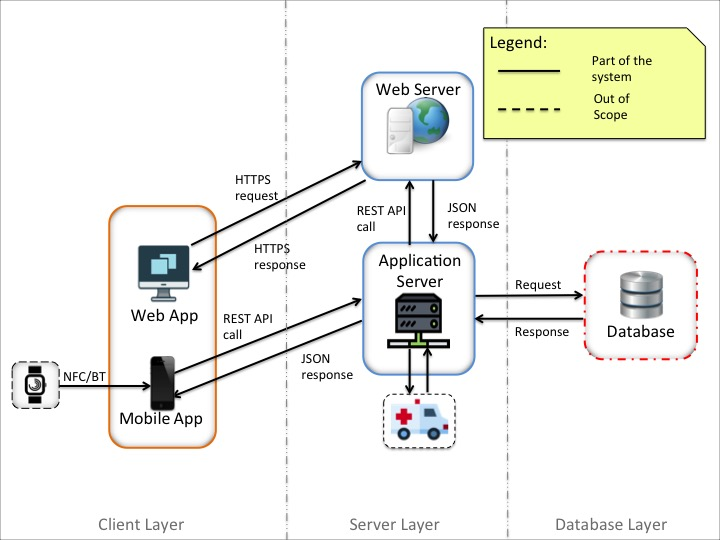
\includegraphics[width=0.85\textwidth,keepaspectratio]{images/highlevel.jpg}
    	\caption{High Level interaction diagram}
\end{figure}
\begin{itemize}
    \item The \textit{Mobile Application} may be connected with an external device such as smart-watches, specific pathology's monitoring devices or other types of external devices able to monitor health parameters with BT or NFC connection;
    \item The \textit{Application Server} should be able to communicate with dispatchers in order to send them individual's position and notify them in case of accident.
\end{itemize}
\hfill
\begin{figure}[!htpb]
    	\centering
    	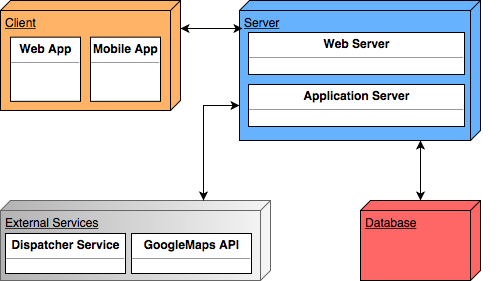
\includegraphics[width=80mm]{images/highlevel2.png}
    	\caption{High Level components diagram}
\end{figure}
\newpage
\subsection{Component View}
    \subsubsection{Application Layer (Server Layer)}
    \paragraph{Authenticator Controller:}
    receives guests' registration and login requests and forward them to the lower layer and also handles users' credentials and profile data management.
    
    \paragraph{Individuals Data Controller:}
    is responsible of individuals' personal data management.
    
    \paragraph{Request Controller:}
    allows to generate individual and group requests. Furthermore it is encharged of the management of incoming request for individuals and of outgoing requests in case of third party users.
    
    \paragraph{Automated-Sos Controller:}
    allows both individual and Third-Party to enable the Sos service. In particular, it allows Individual to chose a Third-Party among the ones that have enabled the Sos service.
    
    \paragraph{Position Controller:}
    is responsible of the communication with the individuals' GPS device in order to get their position through \textit{Google Maps API}.

    \paragraph{Run Controller:}
    handles the creation of a run and allows both Athletes and Spectators to respectively enroll and watch run. This component also handles for organizer definition of the path of the run and, for spectators, watching that run to see athletes position and the predefined path on an interactive map.
    
    \subsubsection{Service Layer (Server Layer)}

    \paragraph{Authenticator Service:}
    handles all the logic related to the login and registration functions. This module receives data from the \textit{User Session Controller}.

    \paragraph{Request Service:}
    is the core component of \textit{Data4Help} logic, it handles all the requests coming from the Data Controller and Request Controller and manages all the Users' private and public data. It validates group and individual requests and return the responses from \textit{Individuals}.
    
    \paragraph{Subscription Service:}
    allows third parties to receive Individual's data as soon they are produced and is in charge of synchronization with new data.
    
    \paragraph{Automated-Sos Service:}
    monitors Individuals' data who activated the service and is able to notify the \textit{Dispatcher} in case of accident.
    
    \paragraph{Run Service:}
    handle runs for creation, enrollment and watching.
    
    \subsubsection{Persistence Layer (Server Layer)}
        
    \paragraph{Health Data Repository:}
    saves and get individuals' health data from the database.
    
    \paragraph{Individual Repository:}
    saves and get individuals' data from the database.
    
    \paragraph{Third Party Repository:}
    saves and get third parties' data from the database.
    
    \paragraph{Request Repository:}
    saves and get only request accepted by \textit{Individuals}.
    
    \paragraph{Automated-Sos Repository:}
    saves users' enabling/disabling of sos services and further accidents data.
    
    \paragraph{Dispatcher Repository:}
    contains dispatchers' data.
    
    \paragraph{Run Repository:}
    saves and get created runs, enrollment and watching information.
    
    \subsubsection{Client Layer}
    
    \paragraph{Google Maps API:}
    used by the client application to create maps through Google Maps services.
    
    \paragraph{External Device API:}
    allows connection with and data acquisition from the Individual external device from a common smart-watch to a specific pathology monitoring device.
    
    \subsubsection{External Services}
    \paragraph{Dispatcher API:}
    used by the Sos service to communicate with ambulances dispatcher.

\newpage
\subsection{Component Interfaces}
\begin{figure}[!htpb]
    \centering
    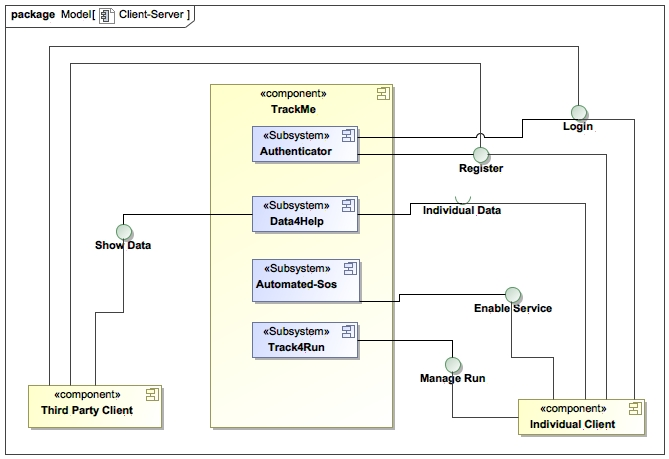
\includegraphics[width=100mm,keepaspectratio]{images/UML/component_TrackMe.jpg}
    \caption{TrackMe Component Diagram}
    \label{fig:component_trackme}
\end{figure}
\begin{figure}[!htpb]
    \centering
    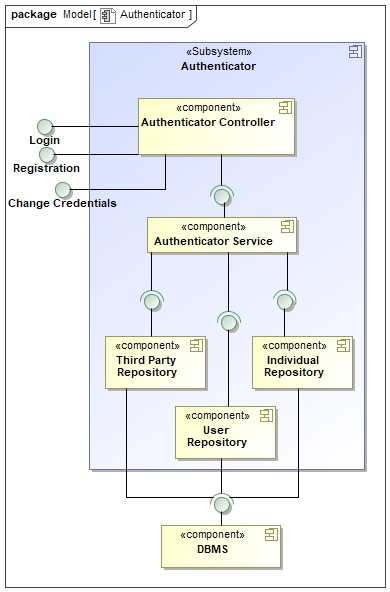
\includegraphics[width=50mm,keepaspectratio]{DD/images/UML/component_Authenticator.jpg}
    \caption{Authenticator Component Diagram}
    \label{fig:component_authenticator}
\end{figure}
\begin{figure}[!htpb]
    \centering
    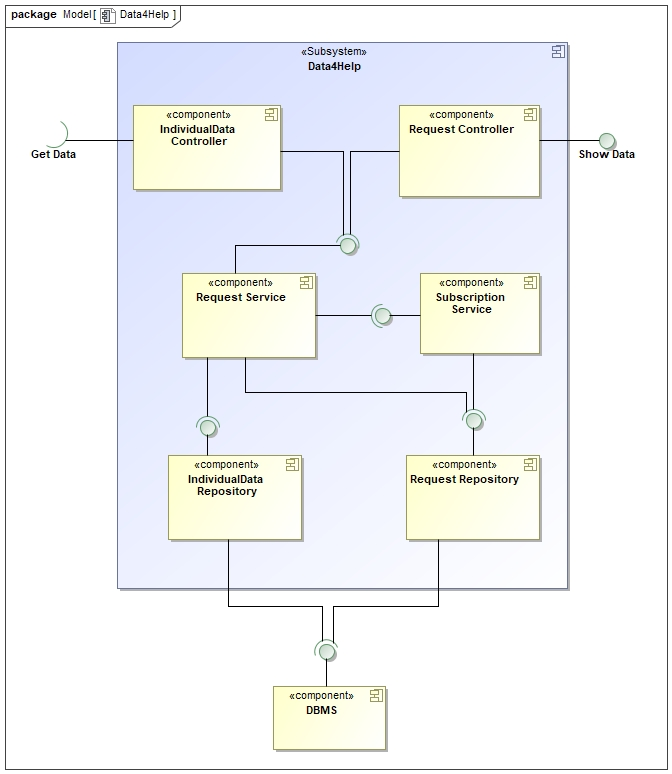
\includegraphics[width=100mm,keepaspectratio]{DD/images/UML/component_Data4Help.jpg}
    \caption{Data4Help Component Diagram}
    \label{fig:component_data4help}
\end{figure}
\begin{figure}[!htpb]
    \centering
    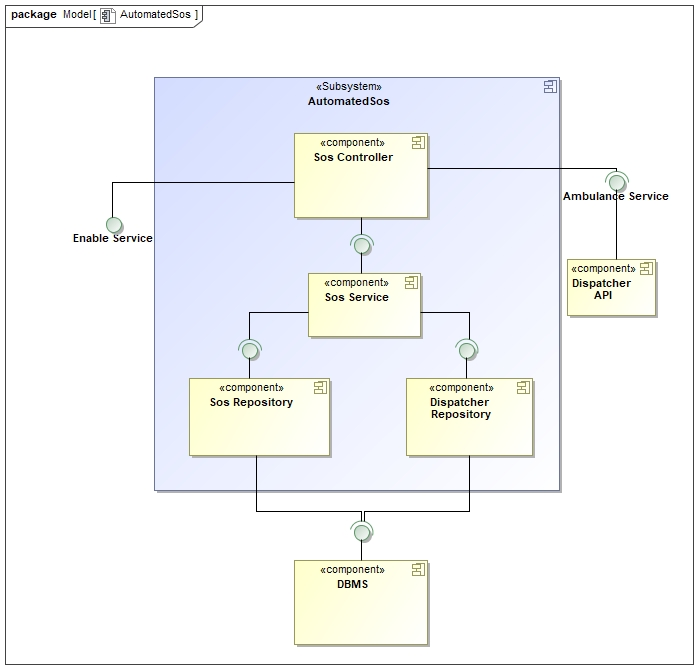
\includegraphics[width=80mm,keepaspectratio]{DD/images/UML/component_AutomatedSos.jpg}
    \caption{AutomatedSos Component Diagram}
    \label{fig:component_automatedsos}
\end{figure}
\begin{figure}[!htpb]
    \centering
    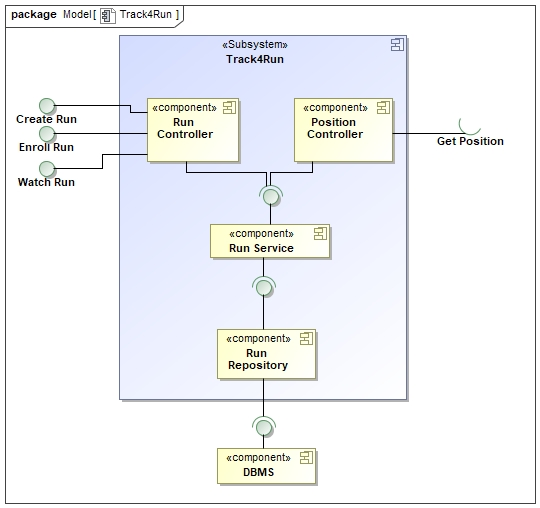
\includegraphics[width=60mm,keepaspectratio]{DD/images/UML/component_Track4Run.jpg}
    \caption{Track4Run Component Diagram}
    \label{fig:component_track4run}
\end{figure}
\begin{figure}[!htpb]
    \centering
    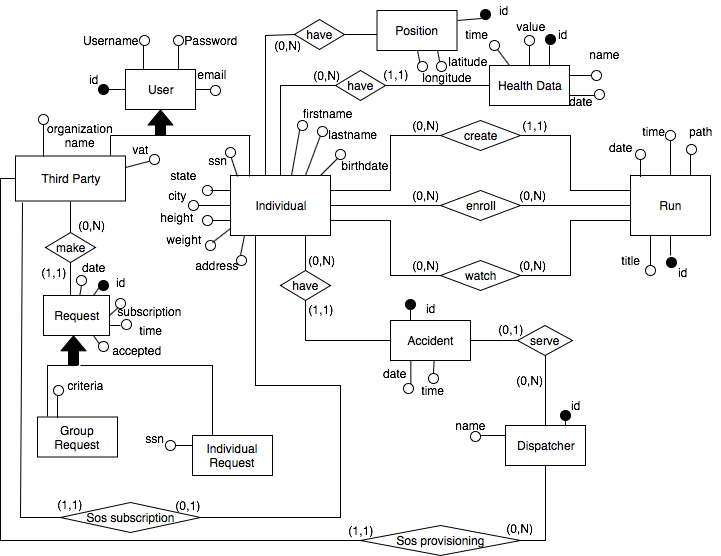
\includegraphics[width=\textwidth,keepaspectratio]{DD/images/er_diagram.png}
    \caption{ER Diagram}
    \label{fig:ER_trackme}
\end{figure}
\newpage
\subsection{Deployment View}
\begin{figure}[!htpb]
    \centering
    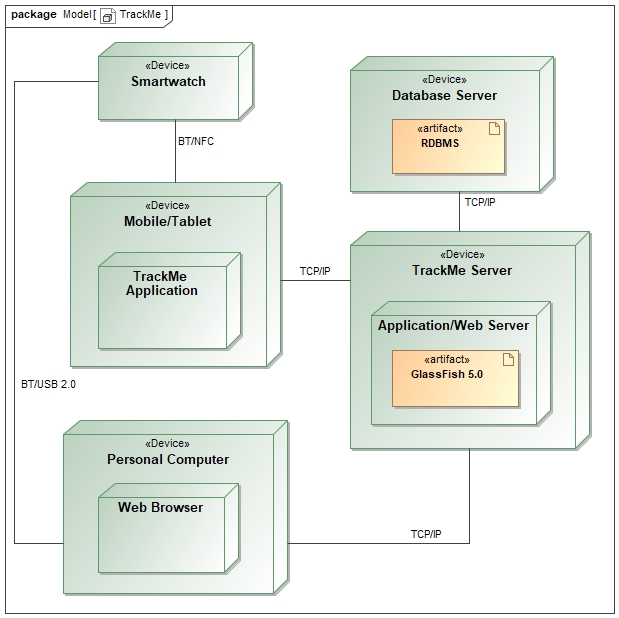
\includegraphics[width=80mm,keepaspectratio]{images/UML/deployment_TrackMe.jpg}
    \caption{TrackMe Deployment Diagram}
    \label{fig:deployment_trackme}
\end{figure}    

\subsection{Class Diagram}
\begin{figure}[!htpb]
    \centering
    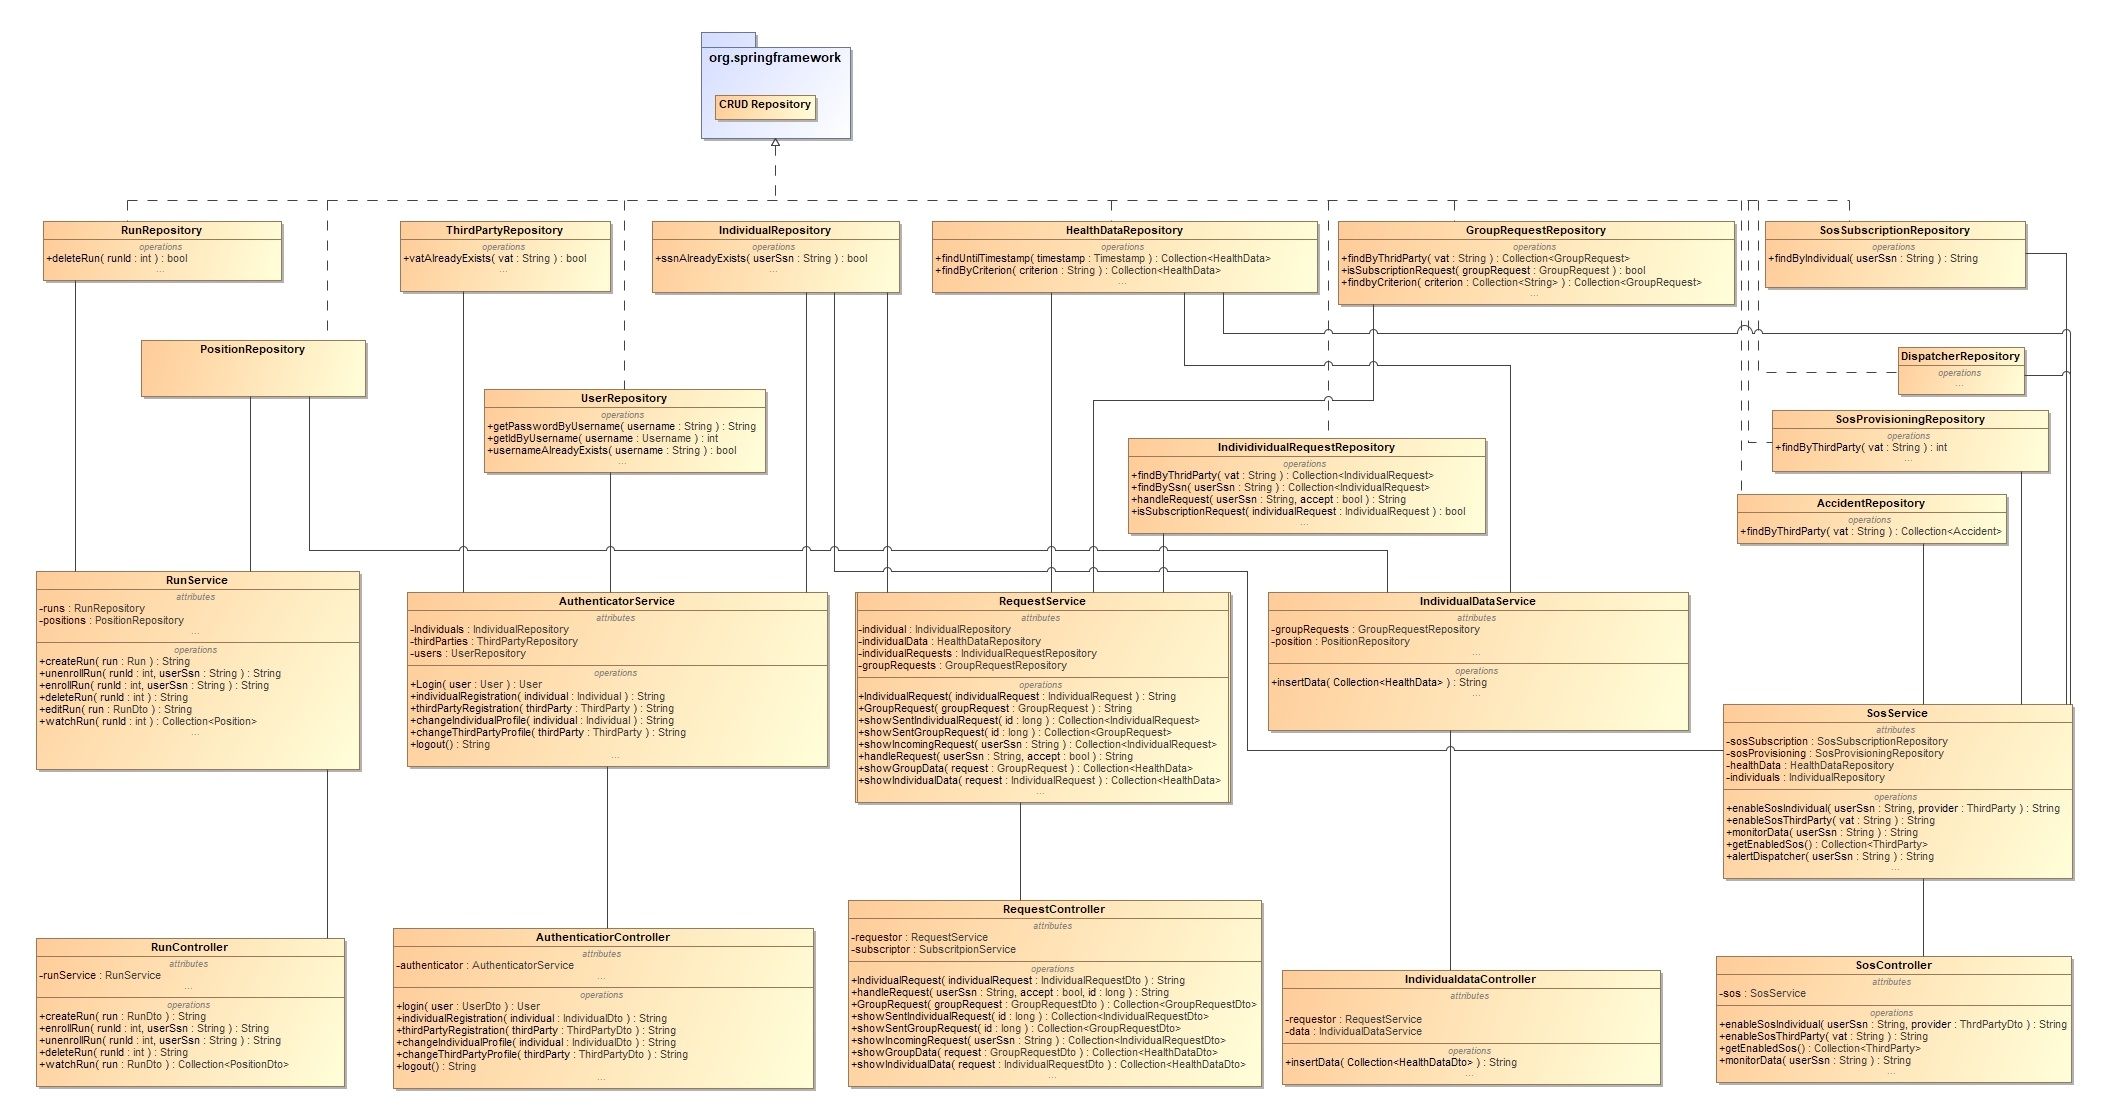
\includegraphics[width=180mm,keepaspectratio,angle=90]{DD/images/UML/ClassDiagram.jpg}
    \caption{Class Diagram}
    \label{fig:CD_trackme}
\end{figure}

\begin{figure}[!htpb]
    \centering
    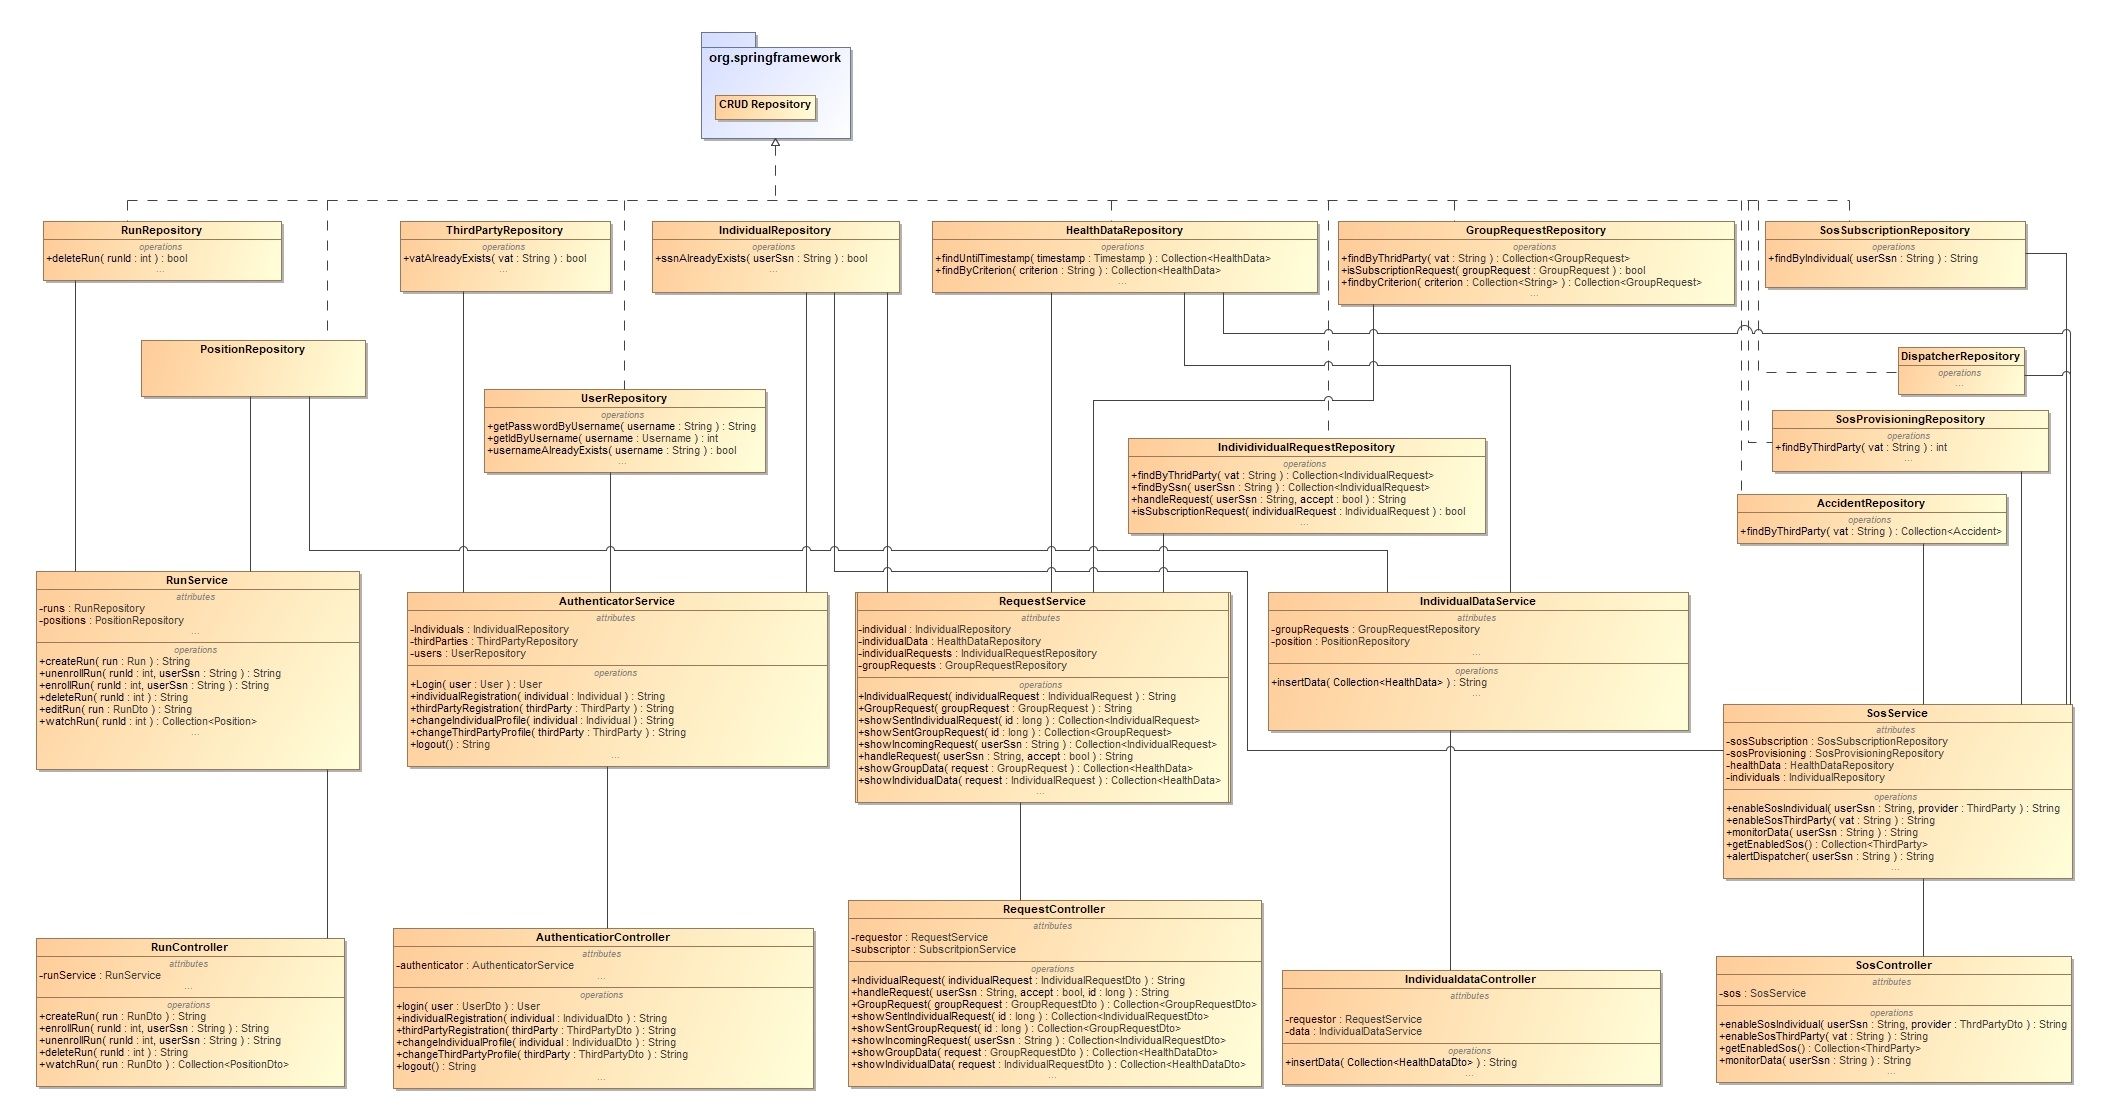
\includegraphics[width=\textwidth,keepaspectratio]{DD/images/UML/ClassDiagram.jpg}
    \caption{Class Diagram: entities}
    \label{fig:CDentities_trackme}
\end{figure}
    
\newpage
\subsection{Runtime View}
\begin{figure}[!htpb]
    \centering
    \advance\leftskip-3cm
    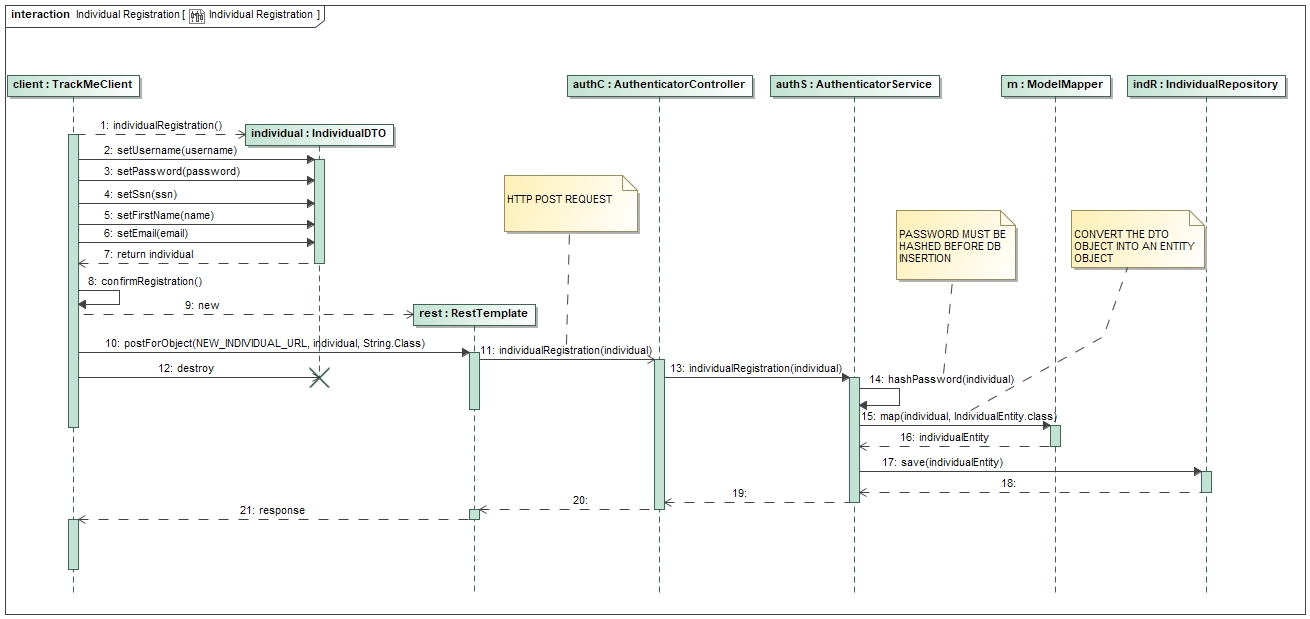
\includegraphics[width=1.5\textwidth,keepaspectratio]{DD/images/UML/sequence_individualRegistration.jpg}
    \caption{Individual Registration Sequence Diagram}
    \label{fig:sequence_individualsignup}
\end{figure} 
\begin{figure}[!htpb]
    \centering
    \advance\leftskip-3cm
    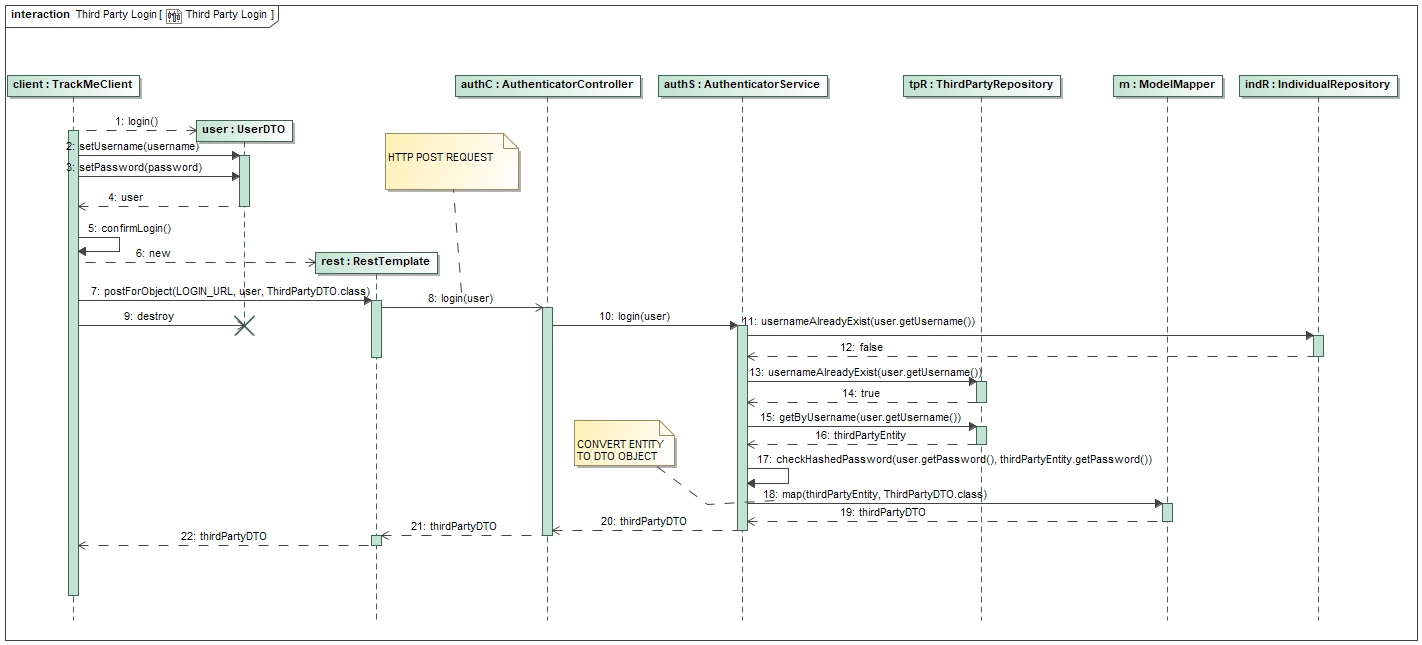
\includegraphics[width=1.5\textwidth,keepaspectratio]{DD/images/UML/sequence_thirdPartyLogin.jpg}
    \caption{Third Party Login Sequence Diagram}
    \label{fig:sequence_tplogin}
\end{figure} 
\begin{figure}[!htpb]
    \centering
    \advance\leftskip-3cm
    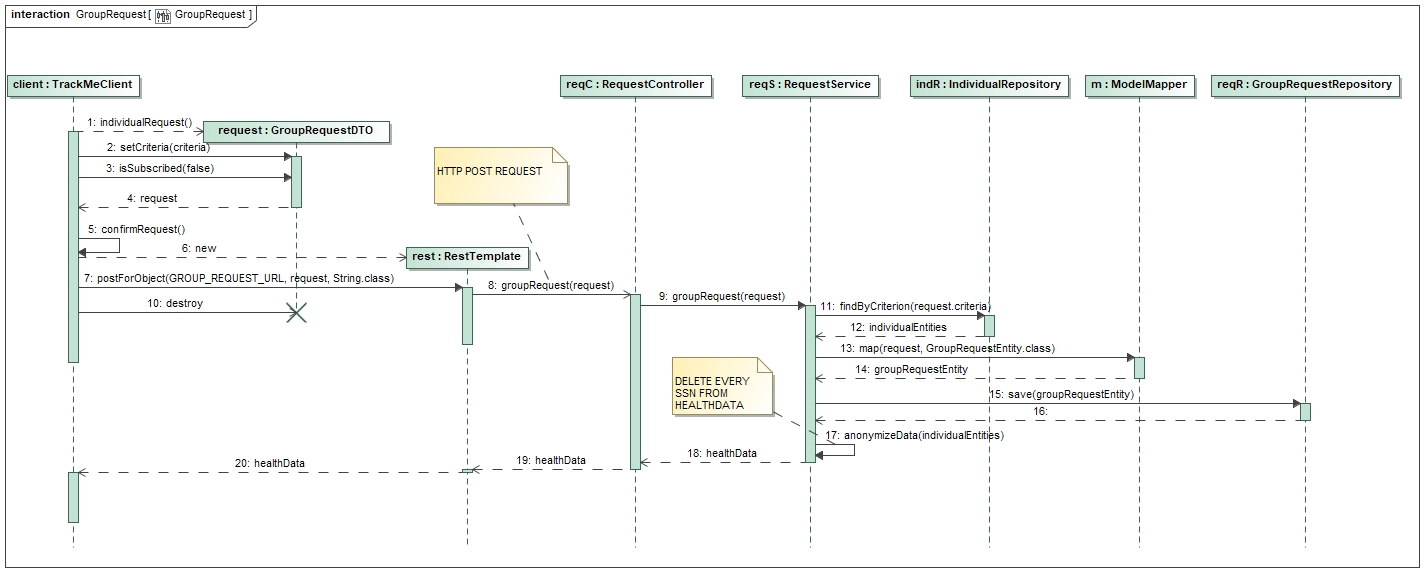
\includegraphics[width=1.5\textwidth,keepaspectratio]{DD/images/UML/sequence_groupRequest.jpg}
    \caption{Group Request Sequence Diagram}
    \label{fig:sequence_grouprequest}
\end{figure}
\begin{figure}[!htpb]
    \centering
    \advance\leftskip-3cm
    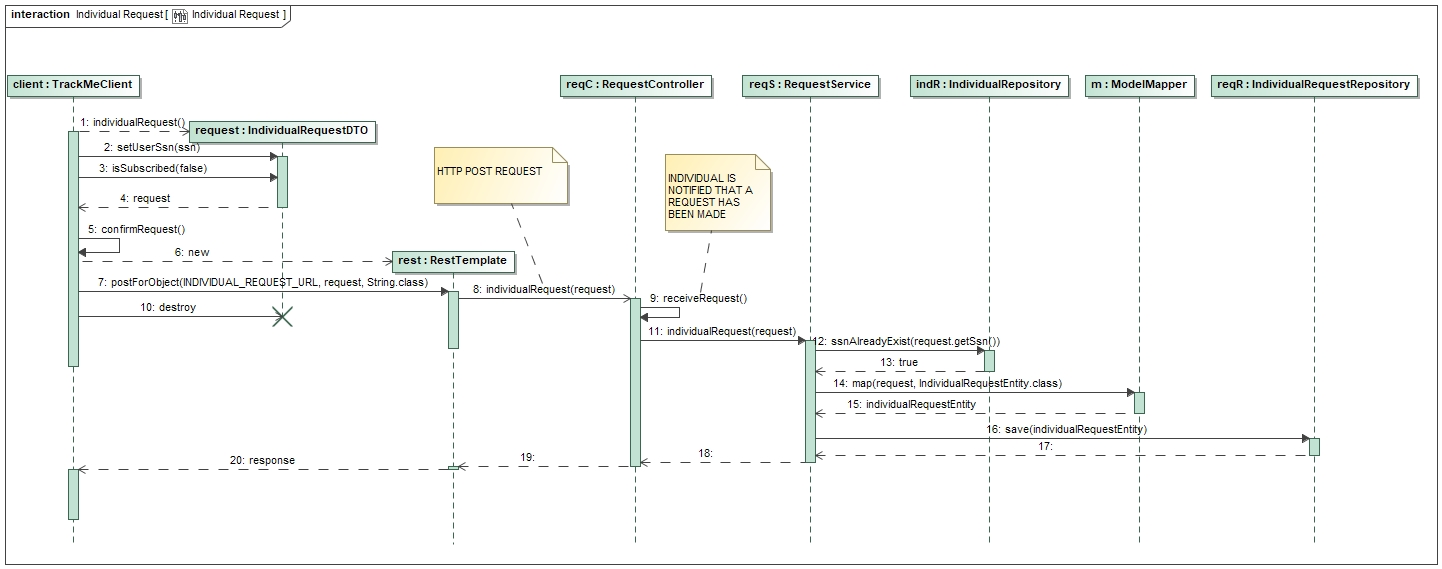
\includegraphics[width=1.5\textwidth,keepaspectratio]{DD/images/UML/sequence_individualRequest.jpg}
    \caption{Individual Request Sequence Diagram}
    \label{fig:sequence_individualrequest}
\end{figure} 
\begin{figure}[!htpb]
    \centering
    \advance\leftskip-3cm
    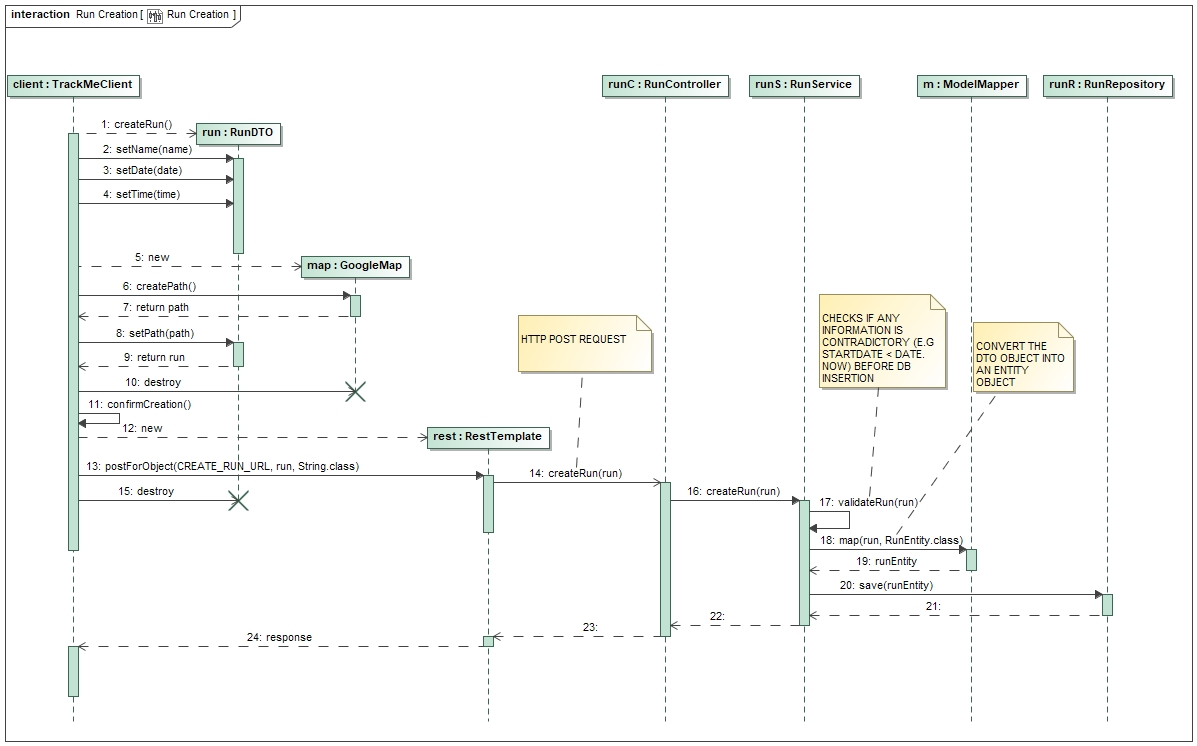
\includegraphics[width=1.5\textwidth,keepaspectratio]{DD/images/UML/sequence_runCreation.jpg}
    \caption{Create Run Sequence Diagram}
    \label{fig:sequence_createrun}
\end{figure}

\newpage
\subsection{Selected Architectural Styles and Patterns}
    \subsubsection{Architecture}
    In order to implement such architecture, based on RESTful API, the following architectural style and design pattern should be taken into account:
    \begin{description}
        \item[Three Tier Architecture:] as showed previously in this document, the layered architecture pattern allows to separate the presentation from the business logic and to realize a thin client with only the user interfaces and input forms and a more complex server that handles all the software services.
        The overall architecture is structured as a three tier architecture: the \textit{Client Layer}, the \textit{Server Layer} and the \textit{Database Layer}.
        
        \item[Layered Server:] The main component of the system is the Server Layer, that it's also deployed on three different layers: the \textbf{Application Layer}, the \textbf{Service Layer} and the \textbf{Persistence Layer}.
        These layers are respectively mapped on the three main components of the software application: \newline controllers, services and repositories.
        \begin{figure}[!htpb]
            	\centering
            	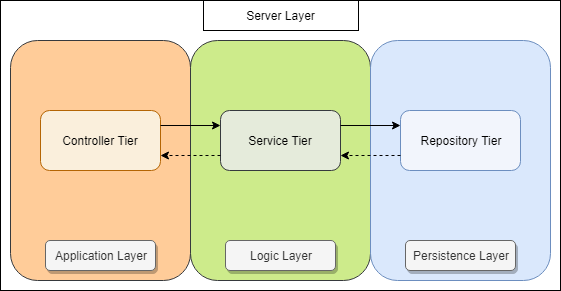
\includegraphics[width=0.84\textwidth,keepaspectratio]{DD/images/ServerLayer.png}
            	\caption{Server Layer diagram}
        \end{figure}
        \newline
        The \textbf{Application Layer} communicates directly with client browser and mobile application, while the \textbf{Service Layer} manages all the application logic: the latter is invoked by the Application Layer. \\
        Lastly the \textbf{Persistence Layer}: here the application has all the database management logic and is responsible of the communication with the DBMS. This layer is invoked by the Logic Layer.\\
        This was done to add \textbf{separation of concerns}: each layer is specialized in a specific activity.
        
        \newpage
        \item[Model View Presenter (MVP):] in this pattern there are three entities: the \textit{Model} which essentially maintains all the data, the \textit{View} that is responsible of showing the model's data and routes user commands to the presenter, and finally the \textit{Presenter} that is responsible of handling the data access from \textit{Model} and to format it to display in the view.
        This architecture is used in the \textit{Client Layer}.
        \begin{figure}[!hb]
            \centering
            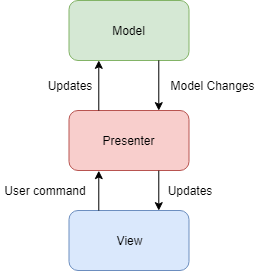
\includegraphics[height=50mm, keepaspectratio]{DD/images/mvp.png}
            \caption{MVP Architecture}
            \label{fig:mvp}
        \end{figure}
    \end{description}
    \subsubsection{Design Patterns}
    \begin{description}
    \item[Publisher-Subscriber:] this is the most important pattern that is used in the application. It is used for almost anything from handling \textit{Data4Help} requests to send athlete positions to spectators through \textit{Track4Run}.
    \begin{figure}[!hb]
        \centering
        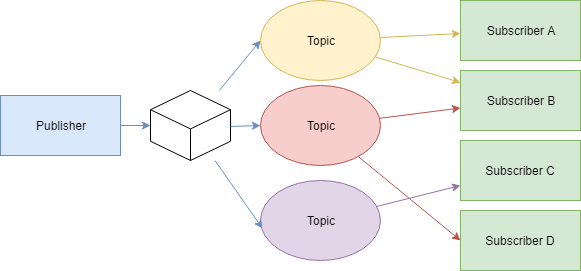
\includegraphics[width=0.9\textwidth,keepaspectratio]{DD/images/pubsub.png}
        \caption{Pub/Sub Pattern}
        \label{fig:pubsub}
    \end{figure}
    
    This is necessary for performance reasons: \textit{TrackMe} is a data-intensive real-time system, so \textit{polling} is not a viable strategy in this case.
    \textit{WebSockets} are clearly the best solution and this is why this pattern shall be used.\\
    Suppose a scenario where a Third Party wants to subscribe to the data of an Individual named Pippo. When Pippo registers to the application, \textit{TrackMe} creates a \textit{topic} associated with him. The Third Party becomes a subscriber of that topic: every time Pippo (Publisher) upload his data, the associated topic is updated and all Third Parties subscribed to him (Subscriber) are notified.
    \end{description}

\subsection{Other Design Decisions}
\subsubsection{Client Localization}
The management of the external device is a client only operation that will allow the application to get Individual's personal health data from the smart device and send them to the server in a lightweight format (e.g. JSON).\\ 

The client map of the run is \textit{local} too: the run organizer will be able (through Google Maps API) to draw a path on an interactive map and send it to the server which will be able to decode the run path and store it as a string; also spectators will be able to use a map to see athletes positions and again, the map will be local too. The Server will provide only athlete positions with the associated track.

\subsubsection{Client Native Application}
In order to allow the user to exploit all the functions of \textit{TrackMe}, the mobile app should be developed for native \textit{Android}/\textit{iOS}. This is necessary for performance reasons.\textit{TrackMe} is a real-time system that relies heavily on data transfer where performance must be maximized; an \textbf{hybrid application} was considered a bad choice for the following reasons:\\
\begin{itemize}
    \item Slower than native application;
    \item Have to work with a wrapper dependent on a third party platform.
\end{itemize}

\subsubsection{Client Web Application}
In addition, a web application may be further developed in order to allow customers to use \textit{Data4Help} features also from their Personal Computers; \textit{Automated-Sos} and \textit{Track4Run} services will instead be available only on mobile devices.

\subsubsection{Programming Languages and Frameworks}
In this design document we assumed the developer is using Java as program-\newline ming language and in particular is deploying the application server through Spring Framework. The rationale for this choice is that this framework fits very well the architectural style of the proposed software solution, has proprietary implementation of the Model View Controller design patter and of several APIs and is very suitable for both provisioning and consuming RESTful services. \\

The choice of using Java and Spring is not a full restriction on the deployment process. In a decision to use a different programming language or to not use Spring Framework would occur, due to the proprietary implementation of several classes, such as the persistence API or the Spring MVC ones, some adaptions to the class diagram may be needed.

\newpage
\section{User Interface Design}
As specified in RASD there are two different user interfaces, one for mobile application and one for web browsers. In this specification we assume the web version of the application will be the same as the mobile application with reduced functions.

\subsection{Mockups}
The guest who access to the main page can sign-up to the application providing his credentials. Once clicked on the \textit{Sign On} button the guest can decide whether registers as an Individual or as a Third-Party, swiping left and right to choose the wright option. Once registered, on the initial page, an user can sign-in in the application inserting Username and Password in the relative boxes and clicking on the \textit{Sign In} button. 

\begin{figure}[!htpb]
    	\centering
    	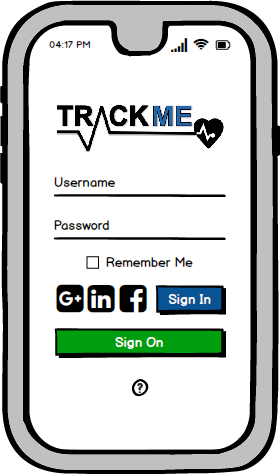
\includegraphics[height=50mm]{images/mockups/Login_Registration.png}
    	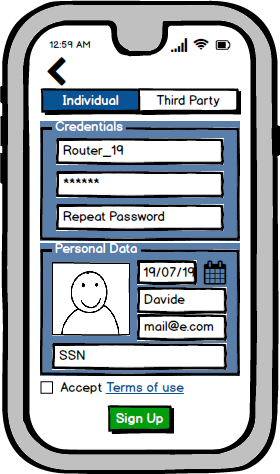
\includegraphics[height=50mm]{DD/images/mockups/IndividualRegistration.png}
    	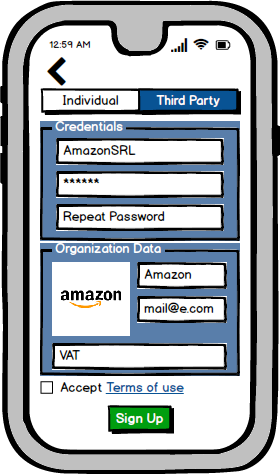
\includegraphics[height=50mm]{images/mockups/ThirdPartyRegistration.png}
        \end{figure}

Once inside the application, the user is redirected to the home page, where he can see his account data. He can press the top-left menu and navigate from there. Here the user can access to services provided by \textit{Data4help} and can enable \textit{Automated-SOS} service too. Individual can also access to \textit{Track4Run} and \textit{External Devices} section. The Individuals can handle incoming request by accepting or rejecting them on the Manage Request page. 

\begin{figure}[!htpb]
    	\centering
    	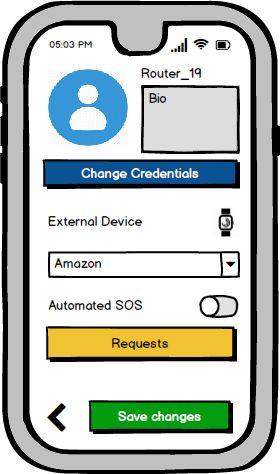
\includegraphics[height=50mm]{images/mockups/IndividualProfile.png}
    	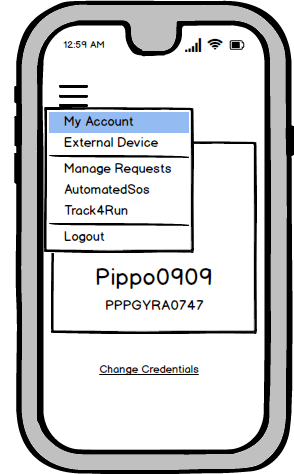
\includegraphics[height=50mm]{images/mockups/IndividualProfileOpen.png}
    	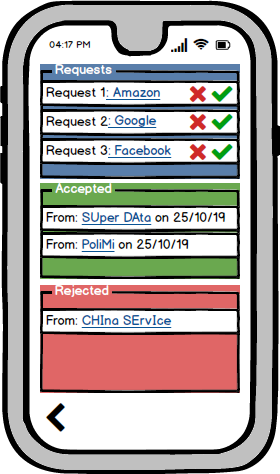
\includegraphics[height=50mm]{images/mockups/ManageRequests.png}
\end{figure}

Third-parties can choose either individual or group request and can enable the option to subscribe to new data.

\begin{figure}[!htpb]
    \centering
    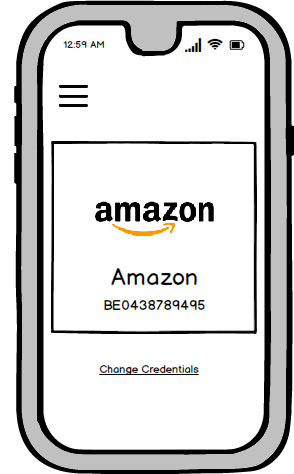
\includegraphics[height=50mm]{images/mockups/ThirdPartyProfile.png}
    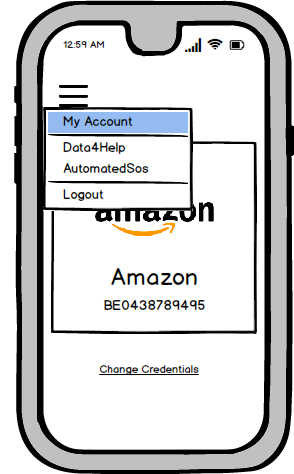
\includegraphics[height=50mm]{images/mockups/ThirdPartyProfileOpen.png}
\end{figure}

The Third- Party, form the Data4Help page, can also reach the view data section: here she can see and plot the data of sent requests. Furthermore, swiping left and right, it can move between individual and group data.
\begin{figure}[!htpb]		
     	\centering		
     	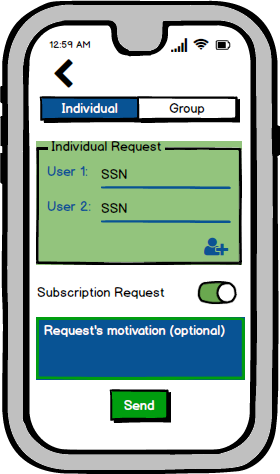
\includegraphics[height=50mm]{images/mockups/Requests.png}		
     	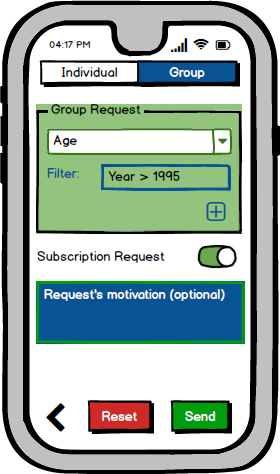
\includegraphics[height=50mm]{images/mockups/GroupRequest.png}		
     	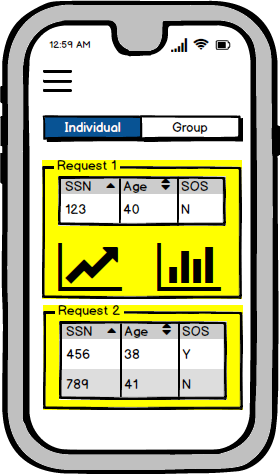
\includegraphics[height=50mm]{images/mockups/ViewData.png}		
     	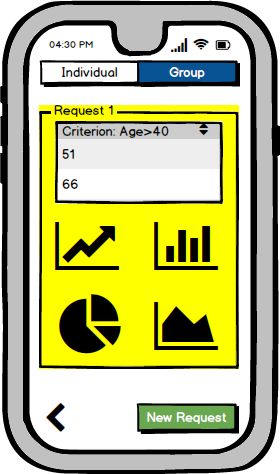
\includegraphics[height=50mm]{images/mockups/ViewData2.png}		
         \end{figure}
        
Once in the \textit{Truck4Run} section, the individual can create, watch, enroll, unroll, start or delete a run.  In the create run page, he can set all the characteristic of the run. Furthermore, he can access to an interactive map to set up the path of the run. In the section watch run there's instead a map with all the position of athletes.

        \begin{figure}[!htpb]
    	\centering
    	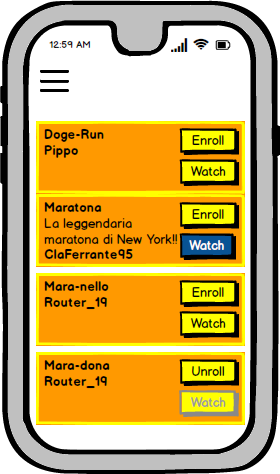
\includegraphics[height=50mm]{images/mockups/RunManager.png}
    	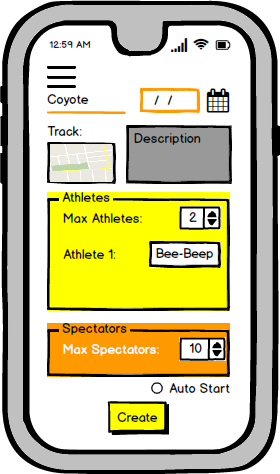
\includegraphics[height=50mm]{images/mockups/RunCreate.png}
    	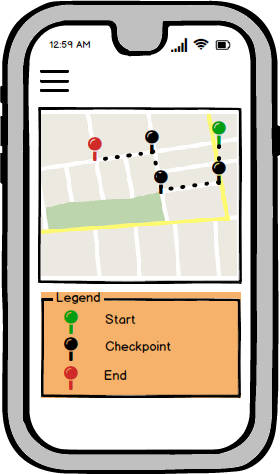
\includegraphics[height=50mm]{images/mockups/DefineTrack.png}
    	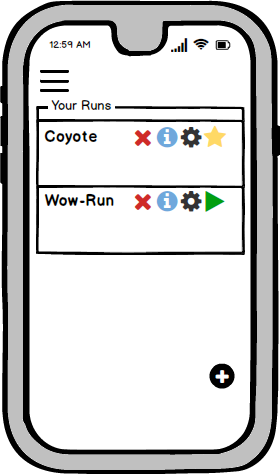
\includegraphics[height=50mm]{images/mockups/MyRuns.png}
        \end{figure}
     \hfill
\subsection{User Experience}
    In this specification we include only mobile users' experience because for web application clients the experience will be the same except for the fact that all \textit{Automated-Sos} and most of \textit{Track4Run} function will be unavailable for web browsers.
    \begin{figure}[!htpb]
    	\centering
    	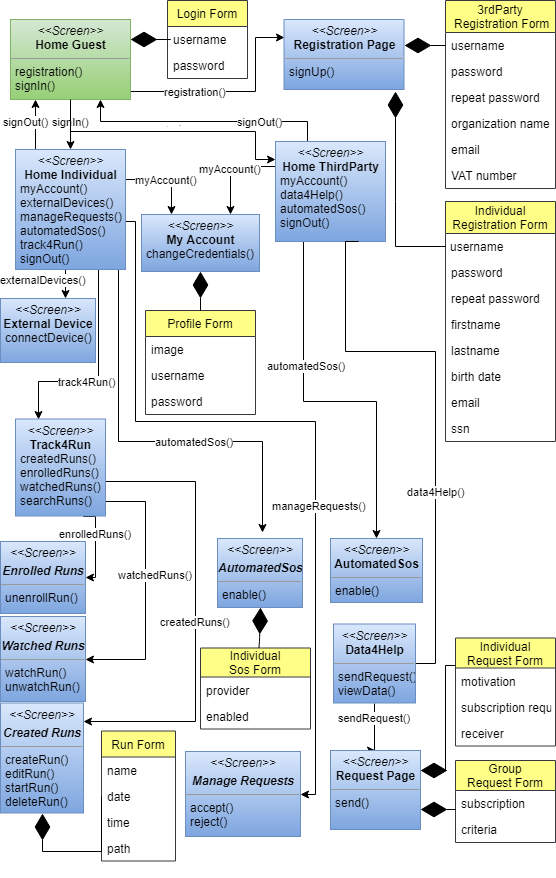
\includegraphics[width=\textwidth, height=0.5\paperheight]{images/ux/ux_TrackMe.png}
    	\caption{User eXperience}
    \end{figure}

\newpage
\section{Requirements Traceability}
\begin{description}
     \con{1}{A customer not signed-on must be able to begin the Individual's registration process to TrackMe providing a username, a password and its organization data.}
    {Authenticator Controller}
    {Authenticator Service}
    {Individual Repository}
     
     \con{2}{A customer not signed-on must be able to begin the Third Party's registration process to TrackMe providing a username, a password and its organization data.}
     {Authenticator Controller}
     {Authenticator Service}
     {Third Party Repository}
    
     \con{3}{The system must provide a log-in interface for already registered users, not previously signed into the application.}
     {Authenticator Controller}
     {Authenticator Service}
     {Individual Repository}
     {Third Party Repository}
     
     \con{4}{TrackMe must provide to users the possibility to change their username.}
     {Authenticator Controller}
     {Authenticator Service}
     {Individual Repository}
     {Third Party Repository}
     
     \con{5}{TrackMe must provide to registered users the possibility to change their password.}
     {Authenticator Controller}
     {Authenticator Service}
     {Individual Repository}
     {Third Party Repository}
     
     \con{6}{The system must provide the possibility to the user of logging out.}
     {Authenticator Controller}
     {Authenticator Service}
     
     \con{7}{The system must provide the possibility to change Individual's personal data.}
     {Authenticator Controller}
     {Authenticator Service}
     {Individual Repository}
     
     \con{8}{The system must provide the possibility to change Third Party's organization data.}
     {Authenticator Controller}
     {Authenticator Service}
     {Third Party Repository}
     
     \con{9}{Data4help must allow the Third-Parties to send a request to a particular individual, provided his SSN/FC.}
     {Request Controller}
     {Request Service}
     {Individual Repository}
     {Individual Request Repository}
     
     \con{10}{Data4help must allow the Third-Parties to generated a request for a group of individuals.}
     {Request Controller}
     {Request Service}
     {Individual Repository}
     {Group Request Repository}
     
     \con{11}{The system must be able to anonymize users' requested data.}
     {Request Controller}
     {Request Service}
     {Individual Repository}
     {Group Request Repository}
     
     \con{12}{Data4help must allow the Third-Parties to choose if subscribe to new data associated with a particular Individual.}
     {Individual Request Controller}
     {Individual Request Service}
     {Request Service}
     {Individual Request Repository}
     {Group Request Repository}


     \con{13}{The system must be able to periodically query the database in order to get new data as soon as they are produced.}
     {Request Controller}
     {Subscription Service}
     {Individual Request Repository}
     {Group Request Repository}
     {Health Data Repository}
     
     \con{14}{Data4help must allow the Third Party to see a list of sent requests and related Individual's data.}
     {Request Controller}
     {Request Service}
     {Individual Request Repository}
     {Health Data Repository}
     
     \con{15}{Data4help must allow the Individual to see a list of the received requests from Third Parties.}
     {Request Controller}
     {Request Service}
     {Individual Request Repository}
     
     \con{16}{Data4help must allow the Individual to accept or reject a request from the list.}
     {Request Controller}
     {Request Service}
     {Individual Request Repository}
     
     \con{17}{Data4help must allow the Individual to connect an external device through BT or NFC.}
     {External Device API}
     
     \con{18}{The system must allow the Third-Party to activate Automated-SOS service.}
     {Sos Controller}
     {Sos Service}
     {Sos Provisioning Repository}
     
     \con{19}{The system must be able to assign an ambulance dispatcher to the SOS service.}
     {Sos Controller}
     {Sos Service}
     {Sos Provisioning Repository}
     {Dispatcher Repository}
     
     \con{20}{The system must allow the Individual to activate Automated-SOS service.}
     {Sos Controller}
     {Sos Service}
     {Sos Subscription Repository}
     {Sos Provisioning Controller}
     
     \con{21}{The system should allow the Individual to choose between third parties who has enabled the service.}
     {Sos Controller}
     {Sos Service}
     {Sos Subscription Repository}
     {Sos Provisioning Controller}
     
     \con{22}{The system must be able to get the Individual position.}
     {Sos Controller}
     {Sos Service}
     {Individual Repository}
     
     \con{23}{The system must be able to send the position to the nearest ambulance.}
     {Sos Controller}
     {Sos Service}
     {Individual Repository}
     {Sos Subscription Repository}
     {Sos Provisioning Controller}
     {Dispatcher Repository}
     
     \con{24}{Track4Run must allow the organizer to create a run with a date, time, duration and a path.}
     {Run Controller}
     {Run Service}
     {Run Repository}
     
     \con{25}{The system must provide an interface that allows the user to define a path on an interactive map.}
     {Google Maps API}
     
     \con{26}{Track4Run must allow the organizer to start a run previously created.}
     {Run Controller}
     {Run Service}
     {Run Repository}
     
     \con{27}{Track4Run must allow the organizer to delete a run previously created.}
     {Run Controller}
     {Run Service}
     {Run Repository}
     
     \con{28}{Track4Run must allow the Athlete to enroll to an already existing run.}
     {Run Controller}
     {Run Service}
     {Run Repository}
     {Enroll Repository}
     
     \con{29}{Track4Run must allow the Athlete to unroll a run.}
     {Run Controller}
     {Run Service}
     {Enroll Repository}
     
     \con{30}{Track4Run must allow the Spectator to see the position of the Athletes on a map during a run.}
     {Position Controller}
     {Run Service}
     {Run Repository}
     {Individual Repository}
     {Watch Repository}
     {Run Repository}

     
\end{description}

\newpage
\section{Implementation, Integration \& Test Plan}
With respect to specific application services, the implementation plan to be followed should be to develop first \textit{Data4Help} functions and then \textit{Automated-Sos} and \textit{Track4Run} facilities, which are built on top of \textit{Data4Help} service.\\

\textit{Authentication} subsystem instead can be implemented independently on the order on which other components are; an implementation strategy for this module is to deploy it in parallel with Data4Help subsystem.

\subsection{Test Strategy}
Despite this document follows a \textit{Top-Down} style starting from an high level point of view to a detailed components and operations description, we advise an \textit{I\&T} plan following the \textit{Bottom-Up} approach, in which modules at lowest layer will be tested first and upper layers will follow then.\\

The unit testing is focused on testing all the software components' features, then the test will proceed to the integration phase: integration of two components will start only after components executing that operations pass the unit test to ensure that the components themselves work fine and that any failure is related to the integration itself.\\

Components to be tested are listed below; integration test will flow from right to left:

\begin{enumerate}

    \item Integration between Authenticator Controller and Service:
    \begin{figure}[!htpb]
    	\centering
    	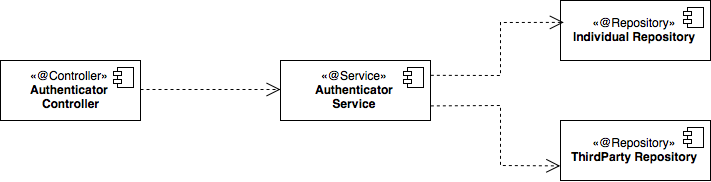
\includegraphics[width=100mm]{images/test/authenticator_integration.png}
    \end{figure}
    
    \item Integration between components of \textit{Data4Help} Subsystem:
    \begin{figure}[!htpb]
    	\centering
    	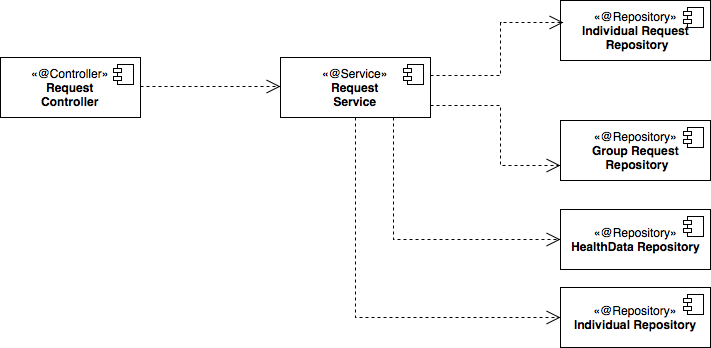
\includegraphics[width=100mm]{images/test/data4help_integration.png}
    \end{figure}
    \newpage
    \begin{figure}[!htpb]
    	\centering
    	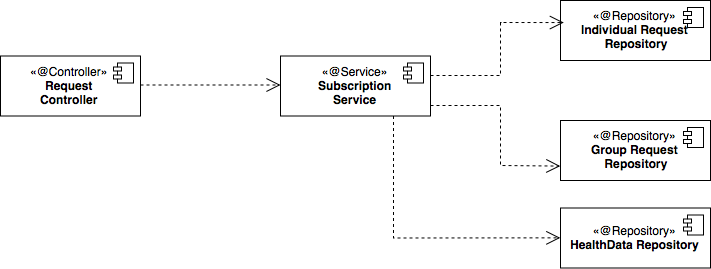
\includegraphics[width=100mm]{images/test/data4help_subscription_integration.png}
    \end{figure}
    
    \item Integration between components of \textit{AutomatedSos} Subsystem:
    \begin{figure}[!htpb]
    	\centering
    	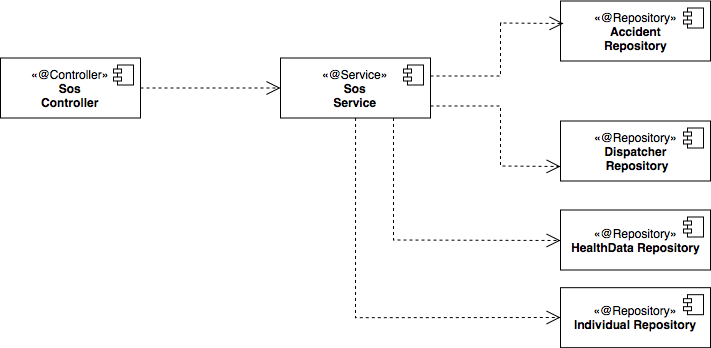
\includegraphics[width=100mm]{images/test/automated_sos_integration.png}
    \end{figure}
    
    \item Integration between components of \textit{Track4Run} Subsystem:
    \begin{figure}[!htpb]
    	\centering
    	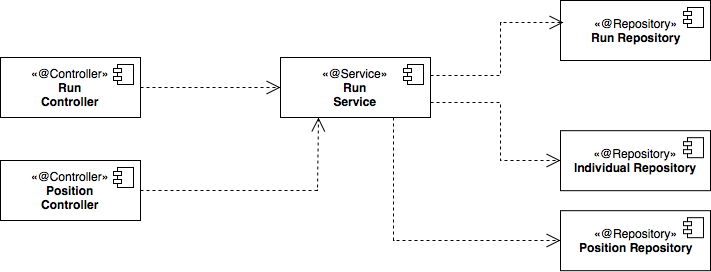
\includegraphics[width=100mm]{images/test/track4run_integration.png}
    \end{figure}
    
\end{enumerate}

\subsection{Entry Criteria}
\subsubsection{Unit Test}
The \textit{Unit Test} phase will start only after:\\
\begin{itemize}
    \item the proposed system architecture has been designed and reviewed;
    \item testable code for units to be tested is available;
    \item the test environment has been properly configured and is ready to run.
\end{itemize}

\subsubsection{Integration Test}
The \textit{Integration Test} phase will start only when:\\
\begin{itemize}
    \item Unit Test phase is completed;
    \item each component has gone through and passed the unit test phase before the integration phase;
    \item all priority bugs found in the unit test phase are fixed and marked as solved;
    \item the test environment has been properly configured and is ready to run.
\end{itemize}

\subsection{Exit Criteria}
\subsubsection{Unit Test}
The \textit{Unit Test} phase will end only after:\\
\begin{itemize}
    \item all unit tests are successfully executed;
    \item priority bugs are fixed.
\end{itemize}

\subsubsection{Integration Test}
The \textit{Integration Test} phase will end only after:\\
\begin{itemize}
    \item integration system has passed all functional requirements;
    \item integration system has passed all performance requirements;
    \item all high severity or top priority bug has been fixed;
    \item high risk identified area has been taken up and tested. \newline
\end{itemize}

If \textit{I\&T} integration exit criteria are satisfied, the test phase can move on to the System Testing in which Load, Performance and Stress tests may be useful to highlight some Quality of Service leaking of the system.

\newpage
\section{Effort Spent}
    \begin{itemize}
        \item[-] \textbf{Davide Rutigliano: 60h}
        
        \item[-] \textbf{Davide Matta: 60h}
        
        \item[-] \textbf{Claudio Ferrante: 60h}
    \end{itemize}

\end{document}